%%%%%%%%%%%%%%%%%
% This is an example CV created using altacv.cls (v1.1.3, 30 April 2017) written by
% LianTze Lim (liantze@gmail.com), based on the 
% Cv created by BusinessInsider at http://www.businessinsider.my/a-sample-resume-for-marissa-mayer-2016-7/?r=US&IR=T
% 
%% It may be distributed and/or modified under the
%% conditions of the LaTeX Project Public License, either version 1.3
%% of this license or (at your option) any later version.
%% The latest version of this license is in
%%    http://www.latex-project.org/lppl.txt
%% and version 1.3 or later is part of all distributions of LaTeX
%% version 2003/12/01 or later.
%%%%%%%%%%%%%%%%

%% If you want to use \orcid or the
%% academicons icons, add "academicons"
%% to the \documentclass options. 
%% Then compile with XeLaTeX or LuaLaTeX.
% \documentclass[10pt,a4paper,academicons]{altacv}

%% Use the "normalphoto" option if you want a normal photo instead of cropped to a circle
% \documentclass[10pt,a4paper,normalphoto]{altacv}

\documentclass[10pt,a4paper]{altacv}

%% AltaCV uses the fontawesome and academicon fonts
%% and packages. 
%% See texdoc.net/pkg/fontawecome and http://texdoc.net/pkg/academicons for full list of symbols.
%% When using the "academicons" option,
%% Compile with LuaLaTeX for best results. If you
%% want to use XeLaTeX, you may need to install
%% Academicons.ttf in your operating system's font %% folder.


% Change the page layout if you need to
\geometry{left=1cm,right=9cm,marginparwidth=6.8cm,marginparsep=1.2cm,top=1cm,bottom=1cm}

% Change the font if you want to.

% If using pdflatex:
\usepackage[utf8]{inputenc}
\usepackage[T1]{fontenc}
\usepackage[default]{lato}
\usepackage{hyperref}

\documentclass{article}
\usepackage{graphicx}
\usepackage{tikz}
\usepackage[margin=1in]{geometry} % Adjust page margins




% If using xelatex or lualatex:
% \setmainfont{Lato}

% Change the colours if you want to
\definecolor{VividPurple}{HTML}{14149c}
\definecolor{SlateGrey}{HTML}{2E2E2E}
\definecolor{LightGrey}{HTML}{666666}
\colorlet{heading}{SlateGrey}
\colorlet{accent}{VividPurple}
\colorlet{emphasis}{SlateGrey}
\colorlet{body}{LightGrey}

% Change the bullets for itemize and rating marker
% for \cvskill if you want to
\renewcommand{\itemmarker}{{\small\textbullet}}
\renewcommand{\ratingmarker}{\faCircle}




%% sample.bib contains your publications
\addbibresource{sample.bib}

\begin{document}
\name{Khalit Hartmann}
\tagline{Freelance Full-Stack Software Engineer}
% Cropped to square from https://en.wikipedia.org/wiki/Marissa_Mayer#/media/File:Marissa_Mayer_May_2014_(cropped).jpg, CC-BY 2.0







\begin{tikzpicture}[remember picture, overlay]
    \node[anchor=north east] at ([xshift=-2.2cm, yshift=-1.6cm]current page.north east) {
        \begin{tikzpicture}
            \node at (0,0) {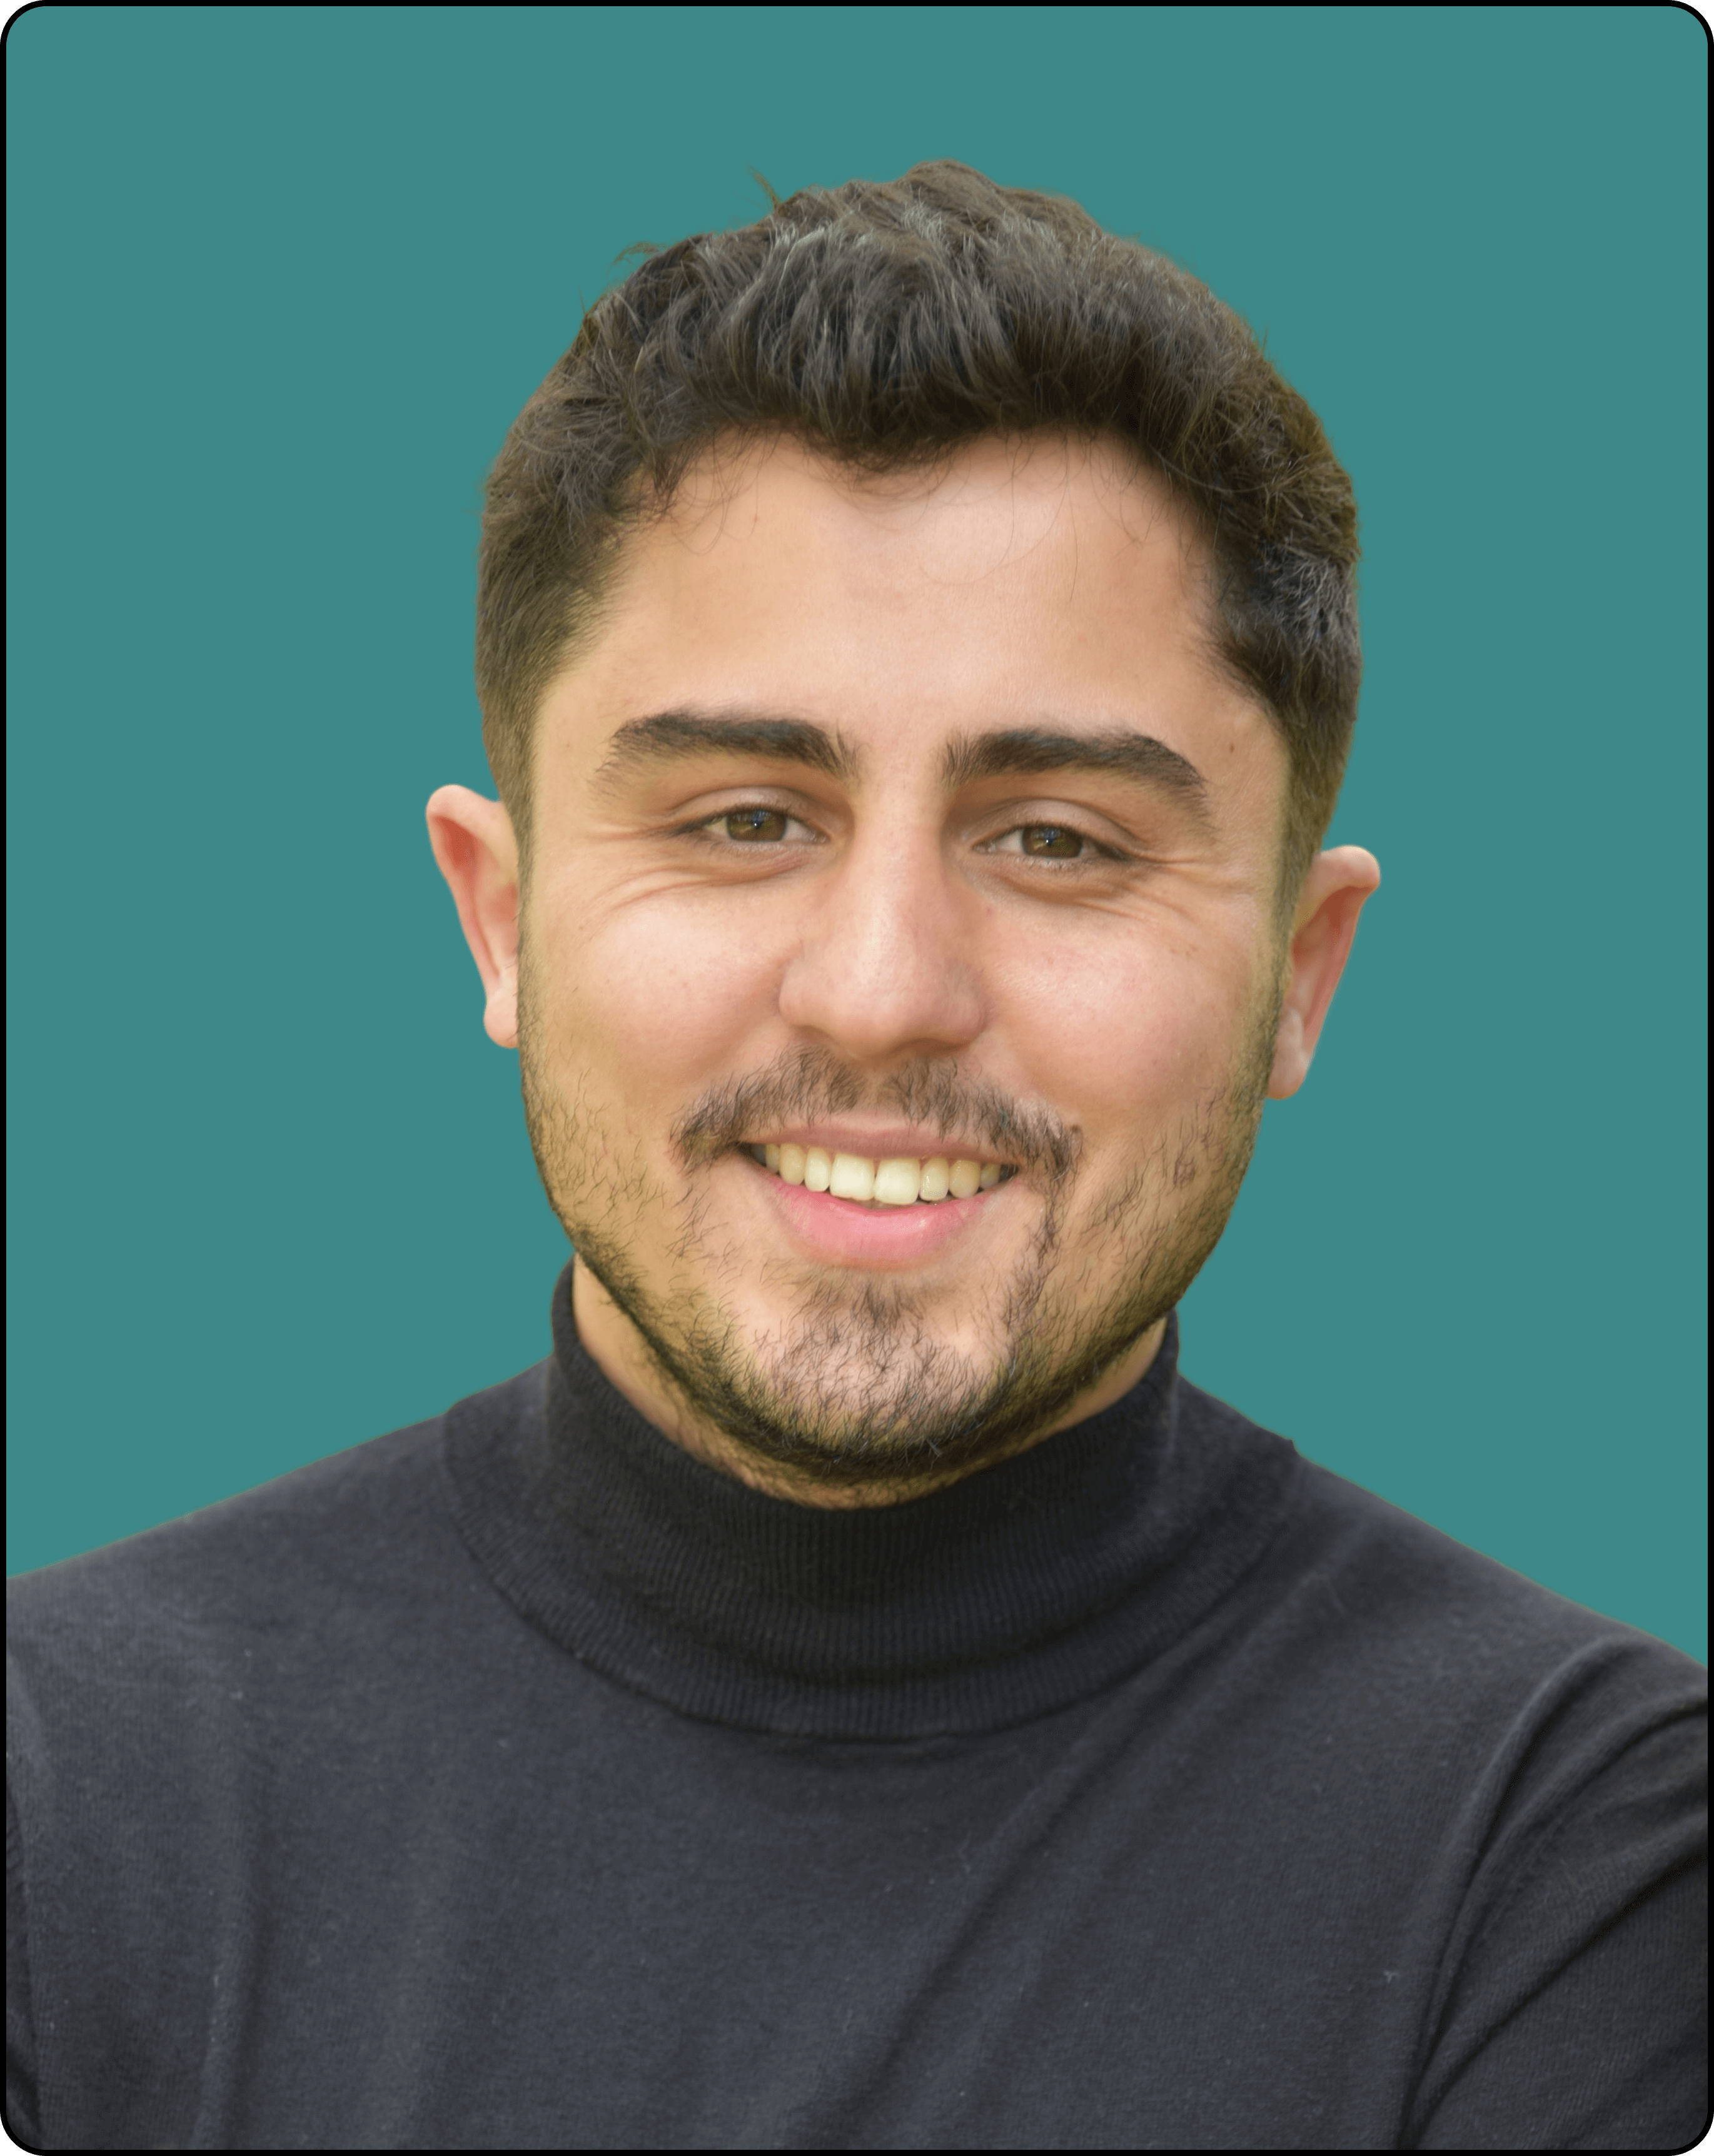
\includegraphics[width=4cm]{khalit.jpeg}}; % Adjust image size
        \end{tikzpicture}
    };
\end{tikzpicture}





\personalinfo{%
  \printinfo{\faHome}{https://khal.it/}
  \newline
  \printinfo{\faGithub}{https://github.com/khal-it}
  \newline
  \printinfo{\faLinkedinSquare}{https://www.linkedin.com/in/khalit-hartmann-7a0356180/}
  \newline
  
  \email{development@khal.it}
  \newline
  \phone{+49 176 233 680 34} 
  \newline
  \location{Berlin}
}

%% Make the header extend all the way to the right, if you want.
\begin{fullwidth}
\makecvheader
\end{fullwidth}


%% Provide the file name containing the sidebar contents as an optional parameter to \cvsection.
%% You can always just use \marginpar{...} if you do
%% not need to align the top of the contents to any
%% \cvsection title in the "main" bar.
\cvsection[page1sidebar]{Experience}





\cvevent{Freelance Team Lead - Mobile App Development}{\href{https://snapnext.de/}{SnapNext GmbH}}{01.08.2024 - 01.03.2025}{}
\begin{itemize}



As a Freelance Mobile Development Lead at SnapNext GmbH, I led a team of two mobile developers to implement new features and maintain Homodea's 2 Apps , focusing on performance, user satisfaction, and revenue growth. Key achievements included a significant increase in daily subscriptions within three months, boosted user engagement through OneSignal push notifications, and the addition of a podcast feature for the Medi app. Together, we implemented in-app messaging, notifications, and promotions, streamlined workflows, integrated Maestro for automated testing, resolved over 70 support tickets, and improved the codebase for scalability and maintainability.
\newline
\newline

\cvtag{Health \& Lifestyle}
\cvtag{Team Leadership}
\cvtag{Growth Hacking}
\cvtag{Push Notifications}
\cvtag{One Signal}
\cvtag{In App Notifications}
\cvtag{Automated Testing}
\cvtag{Architecture}
\cvtag{Flutter}
\cvtag{Dart} 
\cvtag{Docker}
\cvtag{Python}
\cvtag{GraphQL}
\cvtag{Firebase}
\cvtag{Sentry}
\cvtag{Google Analytics}
\cvtag{CI CD}
\cvtag{WebRTC}
\cvtag{SRTP}
\cvtag{iOS}
\cvtag{Android}
\cvtag{Postgress}




\newline
\end{itemize}

\cvevent{Freelance App Developer}{\href{https://www.on.com/en-de/}{On AG}}{01.03.2024 - 01.08.2024}{}
\begin{itemize}



As a freelancer at On AG, I spearheaded the Co-Pilot initiative within the ON App. This initiative focused on exploring and implementing an AI-powered Co-Pilot designed to elevate the overall user experience. The primary objective was to seamlessly integrate advanced AI features into the app, enabling users to interact more intuitively and efficiently. By leading this project, I was responsible for overseeing its strategic development, collaborating with cross-functional teams, and ensuring the Co-Pilot feature aligned with the company's vision of innovation and user-centric design.

\newline
\newline

\cvtag{E-Commerce}
\cvtag{Flutter}
\cvtag{Dart} 
\cvtag{Firebase}
\cvtag{Sentry}
\cvtag{Google Analytics}
\cvtag{Strapi}
\cvtag{REST}
\cvtag{LLM}
\cvtag{Automated Testing}
\cvtag{AI}
\cvtag{Docker}
\cvtag{Contentful}
\cvtag{iOS}
\cvtag{Android}
\cvtag{\href{https://www.on.com/en-de/explore/mobile-app}{On App}}


\newpage
\begin{fullwidth}
    

\cvevent{Freelance App Developer}{\href{https://www.roodie-health.com/}{Roodie Health GmbH}}{01.10.2023 - 01.03.2024}{}






As a freelancer at Roodie Health GmbH, I implement and maintained new features of the Roodie Health App. My role involves ensuring code cleanliness and implementing new features. I worked closely with the client, provided regular updates, and delivered high-quality code. 
\newline
\newline

\cvtag{Health Tech}
\cvtag{Flutter}
\cvtag{Dart} 
\cvtag{Google Analytics}
\cvtag{Firebase Cloud Messaging / Push Notifications}
\cvtag{Sentry}
\cvtag{Google Analytics}
\cvtag{Strapi}
\cvtag{REST}
\cvtag{Java}
\cvtag{Spring Boot}
\cvtag{CI CD}
\cvtag{iOS}
\cvtag{Android}
\cvtag{Postgresql}
\cvtag{\href{https://www.roodie-health.com/}{Roodie App}}

\newline
\divider
    

\cvevent{Experienced Flutter Engineer}{\href{https://careers.mediamarktsaturn.com/MMSTech/?locale=en_US}{MediaMarktSaturn Technology GMBH}}{15.09.2022 - 29.02.2024}{}
As a member of the MediaMarktSaturn Technology team, I am responsible for implementing new features for both MediaMarkt and Saturn Apps across their various sales lines. Working in a team of more than 30 individuals, which includes developers, UI/UX designers, product owners, and stakeholders, I collaborate to maintain the app's functionality and resolve any issues promptly. In addition, I work on optimizing CI/CD pipelines and deploying apps to ensure seamless operations. Overall, my work plays a crucial role in delivering high-quality digital experiences for our customers.
\newline
\newline

\cvtag{E-Commerce}
\cvtag{Flutter}
\cvtag{Dart} 
\cvtag{Firebase}
\cvtag{Sentry}
\cvtag{Google Analytics}
\cvtag{GraphQL}
\cvtag{TypeScript}
\cvtag{Contentful}
\cvtag{Terraform}
\cvtag{NestJs}
\cvtag{NodeJS}
\cvtag{Google Cloud Platform}
\cvtag{CI CD}
\cvtag{iOS}
\cvtag{Android}
\cvtag{Java}
\cvtag{Kotlin}
\cvtag{\href{https://play.google.com/store/apps/details?id=com.media.markt&hl=en_US&pli=1}{MediaMarkt Germany}}
\cvtag{\href{https://play.google.com/store/apps/details?id=com.media.saturn&hl=en&gl=US}{Saturn}}
\cvtag{\href{https://play.google.com/store/apps/details?id=es.mediamarkt.app&hl=en_US}{MediaMarkt Spain}}
\cvtag{\href{https://play.google.com/store/apps/details?id=nl.com.media.markt&hl=nl&gl=US}{MediaMarkt Netherlands}}
\cvtag{\href{https://play.google.com/store/apps/details?id=com.media.markt&hl=en_US&pli=1}{MediaMarkt Italy}}





\divider

\cvevent{Freelance App Developer}{\href{https://www.framegrabber-medien.com/}{FRAMEGRABBER Medien GmbH}}{01.10.2021 - 01.07.2022}{}
As a freelancer at Framegrabber Medien GmbH, I implemented two media guide Apps - DA Kunsthaus Kinder Spiel and DA Kunsthaus Geschichte. My role involved designing and developing the Apps with interactive location-based features. I worked closely with the client, provided regular updates, and delivered high-quality Apps that exceeded their expectations. 
\newline
\newline

\cvtag{Education}
\cvtag{Flutter}
\cvtag{Dart} 
\cvtag{iOS}
\cvtag{Android}
\cvtag{\href{https://apps.apple.com/de/app/da-kunsthaus-kinderspiel/id6443640116}{DA, Kunsthaus Kinderspiel}}
\cvtag{\href{https://play.google.com/store/apps/details?id=com.framegrabber.gravenhorst_adults_app&gl=US}{DA, Kunsthaus Geschichte}}

\newline
\newline
\divider


\cvevent{Freelance App-/Web Developer}{\href{https://snapnext.de/}{SNAPNEXT GMBH}}{01.06.2020 - 01.09.2021}{}


As a freelancer at SnapNext GmbH, I worked on several exciting projects that involved implementing mobile and web applications for different clients. I was responsible for designing, developing, and delivering high-quality applications that met the clients' needs. Some of the Apps I worked on include the \href{https://bit.ly/3tEGnTf}{\textit{\textbf{Mein Orthomol}}} and \href{https://bit.ly/3DfgH2S}{\textit{\textbf{Orthomol - Virtuelle Apotheke}}} mobile apps, the Tetra Pak  \href{https://tetra-pak-mosaik.web.app/}{\textit{\textbf{ Mosaik}}} and \href{https://tetrapak-dabf7.web.app/}{\textit{\textbf{Tetrapak WEIHNACHTS-ORCHESTER}}} web apps, and the \href{https://bit.ly/3DcJzJ5}{\textit{\textbf{EFFZEH 360}}} Unity App, which I maintained to ensure its smooth operation. Throughout these projects, I worked closely with the clients, providing regular updates and soliciting feedback to ensure that the applications met their expectations.
\newline



\cvtag{Health \& Lifestyle}
\cvtag{E-Commerce}
\cvtag{Flutter}
\cvtag{Dart}
\cvtag{ReactJS}
\cvtag{JavaScript}
\cvtag{CI/CD}
\cvtag{Firebase / Google Analytics}
\cvtag{JAMStack}
\cvtag{Salesforce}
\cvtag{Shopware}
\cvtag{Vue.js}
\cvtag{iOS}
\cvtag{Postgresql}
\cvtag{Android}
\cvtag{Python}
\cvtag{\href{https://www.orthomol.com/de-de/service/app}{Mein Orthomol}}
\newline


\divider

\cvevent{Freelance App Developer}{TRIPPLE-A-CODE GMBH }{15.01.2020 - 01.06.2020}{}

As a freelancer at Triple A Code, I developed the \href{https://bit.ly/3IHeeiF}{\textit{\textbf{Holoswitch - Take your phone to Virtual Reality}}} App and set up a Bitbucket CI/CD pipeline. Working closely with clients, I designed, developed, and delivered high-quality applications that met their needs.
\newline

\cvtag{Virtual Reality}
\cvtag{Flutter}
\cvtag{Dart}
\cvtag{WebRTC}
\cvtag{Virtual Reality}
\cvtag{CI/CD}
\cvtag{WebRTC}
\cvtag{Vue.js}
\cvtag{iOS}
\cvtag{Android}
\cvtag{Java}

\newpage

\cvevent{Team Lead / App Developer}{PEQAS GMBH}{01.11.18 - 01.01.2020}{}
As a working student at Peqas GmbH, I had the opportunity to work on several exciting projects. One of my significant achievements was organizing a team of 5 part-time developers and one designer and leading them to work on a cross-platform mobile application from scratch. Additionally, I set up different environments, Travis CI/CD pipelines, and AWS servers to ensure smooth and efficient application delivery. As a leader, I organized and led weekly sprint meetings to keep the team on track and focused on achieving our goals. Working at Peqas GmbH was a valuable learning experience that allowed me to develop my skills and gain practical experience working in a team environment.
\newline
\newline

\cvtag{Augmented Reality}
\cvtag{Flutter}
\cvtag{Dart}
\cvtag{CI/CD}
\cvtag{TypeScript}
\cvtag{Python}
\cvtag{Firebase}
\cvtag{Agile Project Management}
\cvtag{Vue.js}
\cvtag{SRTP}
\cvtag{iOS}
\cvtag{Android}


\divider

\cvevent{Working Student - Data Scientist}{\href{https://dai-labor.de/}{DAI-Labor – Distributed Artificial Intelligence Laboratory}}{01.03.2018 - 01.11.2018}{}
During my time as a working student at DAI Laboratories, I worked on an event-based recommender system for Realeyz GmbH in collaboration with EYZ-Media GmbH. This involved designing and developing an intelligent system that could recommend movies based on relevant events happening in the world. The system used data analysis and machine learning algorithms to identify events and match them with relevant movies from Realeyz's extensive library.
You can find more Information in this \href{https://eyzmedia.de/en/event-based-approach/}{blog post}.
\newline

\cvtag{Research}
\cvtag{NLP}
\cvtag{Web Scraping}
\cvtag{Spacy}
\cvtag{Scrapy}
\cvtag{Postgresql}
\cvtag{Python}
\cvtag{Java}
\cvtag{Spring Boot}
\newline

\cvsection{My Personal Projects}


\cvevent{Tessellai - Event based }{DAI-Labor – Distributed Artificial Intelligence Laboratory}}{01.03.2018 - 01.11.2018}{}
}{blog post}.
\newline

\end{fullwidth}






%\cvsection{References}
%\begin{itemsize}
%\begin{quote}
%``Wunderbare, professionelle Zusammenarbeit! K. hat den Grundstein für unsere gesamte mobile %App Entwicklung gelegt. Sehr zu empfehlen!! `` - Andre Gröschel, TrippleACode GmbH 
%\newline
%\end{quote}
%\begin{quote}
%``Professionelle, ergebnisorientierte, stets freundliche Zusammenarbeit. Ohne Einschränkung %weiterzuempfehlen. Danke K.! `` - Timo Mugele, Framegrabber GmbH 
%\newline
%\end{quote}

%\begin{quote}
%``K. hat uns mit klarer Kommunikation und vollem Einsatz überzeugt. Wir können die %Zusammenarbeit mit ihm nur empfehlen ``- Tim Schröder, MassiveMiniTeam GmbH
%\newline
%\end{quote}

%\begin{quote}
%``Khalid has both, self-organization and autodidactic knowledge and abilities, thus he is %stepping out, compared to regular flutter developers! `` - Max Arbeiter, SnapNext GmbH 
%\newline
%\end{quote}




%\end{itemsize}


\end{document}
